%%
% قالب استاندارد گزارش‌های درسی و گزارش های پروژه برای دانشگاه علم و صنعت ایران
% تهیه و تدوین: مرتضی ذاکری نصرآبادی
% Morteza ZAKERI NASRABADI
% m-zakeri@live.com

% 
%% نسخه 1.1 (13981125)
% - تغییرات در نسخه 1.1
% -- قابل حمل شدن بخش فونت (بخش فونت بایتسی توسط استفاده کننده درج شود)
% -- سازگاری با TexLive 2018
%
%% نسخه 1.0 (13961025)
%
%
%%
\documentclass[a4paper,12pt]{article}
% در ورژن جدید زی‌پرشین برای تایپ متن‌های ریاضی، این سه بسته، حتماً باید فراخوانی شود
\usepackage{amsthm,amssymb,amsmath}
% بسته‌ای برای تنطیم حاشیه‌های بالا، پایین، چپ و راست صفحه
\usepackage[top=30mm, bottom=30mm, left=25mm, right=30mm]{geometry}
%\usepackage[nottoc,numbib]{tocbibind}
\usepackage[nottoc]{tocbibind}
\usepackage{enumerate}
%\usepackage{bm}
% بسته‌‌ای برای ظاهر شدن شکل‌ها و تعیین آدرس تصاویر
\usepackage[final]{graphicx}
\graphicspath{{./figs/}}
\usepackage{caption}
%\usepackage{subcaption}
%\usepackage{subfig}

\usepackage{float}
\usepackage{xparse}
\usepackage{listing}
\usepackage[final]{listings}
\lstset{inputpath=./codes/}

%\usepackage{color}
\usepackage[usenames,dvipsnames,svgnames,table]{xcolor}
\usepackage{soulutf8}


% بسته‌ لازم برای تنظیم سربرگ‌ها
\usepackage{fancyhdr}
\usepackage{setspace}
% بسته‌های لازم برای نوشتن الگوریتم
\usepackage{algorithm}
\usepackage{algorithmic}
% Add by Morteza %
%\usepackage[linesnumbered,ruled,vlined]{algorithm2e}
% بسته‌های لازم برای رسم بهتر جداول
\usepackage{tabulary}
\usepackage{tabularx}
%% Add by Morteza
\usepackage{multirow}
\usepackage{fourier} 
\usepackage{array}
\usepackage{makecell}  % I use this %
\usepackage{booktabs}

%%
% بسته‌های لازم برای رسم تنظیم بهتر شکل‌ها و زیرشکل‌ها
\usepackage[export]{adjustbox}
%\usepackage{subfigure}

%\usepackage[subfigure]{tocloft}
\usepackage{tocloft}
%\usepackage{subfig}
%\usepackage{caption}
%\usepackage{subcaption}

% بسته‌ای برای رسم کادر
\usepackage{framed} 
% بسته‌‌ای برای چاپ شدن خودکار تعداد صفحات در صفحه «معرفی پایان‌نامه»
\usepackage{lastpage}
\usepackage{cite}	% Add by Morteza %

\usepackage[unicode=true, pagebackref=false, colorlinks, linkcolor=Blue, citecolor=Purple, urlcolor=Red, bookmarks=true, linktocpage, breaklinks]{hyperref}

% بسته‌ٔ لازم برای: ۱. تغییر شماره‌گذاری صفحات پیوست. ۲. تصحیح باگ آدرس وب حاوی '%' در مراجع
\usepackage{etoolbox}
\usepackage{comment}

\usepackage{blindtext}
\usepackage{tcolorbox}

\newtcolorbox{mybox}{boxrule=2pt,width=\textwidth,arc=2mm,colback=gray!1}
\newtcolorbox{mybox2}[2][]{width=\textwidth,colback={green},colbacktitle=yellow,coltitle=blue, title=#2,#1}


%%%%%%%%%%%%%%%%%%%%%%%%%%%%%%%%%%%%%%%%%%%%%%%%%%%%
% فراخوانی بسته زی‌پرشین و تعریف قلم فارسی و انگلیسی
% قلم فارسی بازنویسی و قابل حمل شده است. امکان استفاده از چندین فونت فارسی مختلف در این قسمت فراهم شده است. برای استفاده نیازی به نصب بودن فونت ها روی رایانه خود ندارید.

%\usepackage[extrafootnotefeatures]{xepersian}
\usepackage{xepersian}

\settextfont[Path={./font/Niloofar/}, BoldFont={XBNiloofarBd.ttf}, ItalicFont={XBNiloofarIt.ttf}, BoldItalicFont={XBNiloofarBdIt.ttf}, Scale=1.0]{XBNiloofar.ttf}

\setlatintextfont[Scale=0.90]{Times New Roman}
% چنانچه می‌خواهید اعداد در فرمول‌ها، انگلیسی باشد، خط زیر را غیرفعال کنید
\setdigitfont[Path={./font/Zar/}, BoldFont={XBZarBd.ttf}, ItalicFont={XBZarIt.ttf}, BoldItalicFont={XBZarBdIt.ttf}, Scale=1.0]{XBZar.ttf}

% اگر می‌خواهید که اعداد با فونت یکان نمایش داده شوند خط بالا را غیر فعال کرده و خط زیر را فعال کنید.

%\setdigitfont[Path={./font/Yekan/}, BoldFont={XMYekanBd.ttf}, ItalicFont={XMYekanIt.ttf}, BoldItalicFont={XMYekanBdIt.ttf}, Scale=1.0]{XMYekan.ttf}%{Persian Modern}

% تعریف قلم‌های فارسی و انگلیسی اضافی برای استفاده در بعضی از قسمت‌های متن
\defpersianfont\yagut[Path={./font/Yagut/}, BoldFont={XBYagutBd.ttf}, ItalicFont={XBYagutIt.ttf}, BoldItalicFont={XBYagutBdIt.ttf}, Scale=1.0]{XBYagut.ttf}

\defpersianfont\titlefont[Path={./font/Titre/}, BoldFont={XBTitreShadow.ttf}, ItalicFont={XBTitreIt.ttf}, BoldItalicFont={XBTitreShadowIt.ttf}, Scale=1.0]{XBTitre.ttf}

\defpersianfont\iranic[Path={./font/Zar/XBZarOblique/}, BoldFont={XBZarObliqueBd.ttf}, Scale=1.10]{XBZarOblique.ttf}%Italic}%

\defpersianfont\nastaliq[Path={./font/IranNastaliq/}, Scale=1.50]{IranNastaliq.ttf}

%%%%%%%%%%%%%%%%%%%%%%%%%%
% بسته زیر و متعاقباً دستورات ادامه آن، برای ریست کردن شماره پانویس‌ها در هر صفحه قرار داده شده است (به درخواست دکتر محمد عبداللهی ازگمی)--> رونوشت از پایان‌نامه کارشناسی ارشد

%\usepackage[perpage]{footmisc}
\usepackage{zref-perpage}
\zmakeperpage{footnote}
%%%%%%%%%%%%%%%%%%%%%%%%%%%%%%%%%%%%%%%%%%%%%%%%%%%%

\makeatletter
\newcommand*{\Computebaselinestretch}[1]{%
	\strip@pt\dimexpr\number\numexpr\number\dimexpr#1\relax*65536/\number\dimexpr\baselineskip\relax\relax sp\relax
}
\makeatother
\linespread{\Computebaselinestretch{1.05cm}}

\usepackage{csquotes}
\usepackage{epigraph}
\setlength\epigraphwidth{.7\textwidth}
\renewcommand{\epigraphflush}{flushleft}
\renewcommand{\sourceflush}{flushleft}
\renewcommand{\textflush}{flushepinormal}

%\usepackage{polyglossia}
%\usepackage[algo2e,linesnumbered,ruled,vlined]{algorithm2e}
\usepackage{textgreek}
\usepackage{booktabs}  % professional-quality tables
\usepackage{amsfonts}  % blackboard math symbols
\usepackage{nicefrac}  % compact symbols for 1/2, etc.
\usepackage{microtype}  % microtypography
\usepackage{amsmath}
\usepackage[algo2e, ruled, linesnumbered, resetcount]{algorithm2e}
\def\HiLi{\leavevmode\rlap{\hbox to \hsize{\color{yellow!50}\leaders\hrule height .8\baselineskip depth .5ex\hfill}}}


%%%%%%%%%%%%%%%%%%%%%%%%%%%%%%%%%%%%%%%%%%%%%%%%%%
\newcommand{\faculty}{دانشکده مهندسی کامپیوتر}
\newcommand{\group}{گروه نرم‌افزار}
\newcommand{\eyear}{سال تحصیلی 99-1398}
\newcommand{\semester}{دوم (بهار 1399)}
\newcommand{\course}{شبکه‌های پیچیده پویا}
\newcommand{\lecturer}{دکتر حسین رحمانی}
\newcommand{\teachingassist}{ذاکری - ملکی‌فر}
\newcommand{\term}{دوم (بهار 1399)}
\newcommand{\examnum}{پروژه اول}
\newcommand{\examtopic}{سنجش کیفیت معماری نرم‌افزار}
\newcommand{\sentexamdate}{05/12/1398}
\newcommand{\examdate}{20/12/1398}
\newcommand{\timelimit}{100 دقیقه}
%%%%%%%%%%%%%%%%%%%%%%%%%

\def\BoldTitle{\huge{\course}}

\def\Subtitle{\examnum \\ \textbf{\examtopic}}

\title{
\includegraphics[width=0.25\linewidth]{./logo.pdf}\\{\fontsize{16}{0}\nastaliq{\faculty}} \\ \BoldTitle \\ \large{\Subtitle} \\ }

\author{
	مدرس: \\  \lecturer
 \\کمک مدرس:  \\ \teachingassist
	\\
	 \\  
}

%\title{}
%\author{}
%\date{اسفند 1398}
%\date{}
%%%%%%%%%%%%%%%%%%%%%%%%%%%%%%%%%%%%%%%%%%%%%%%%%%%%


\begin{document}

%\fancyhead[LE,RO]{\slshape \rightmark}
%\fancyhead[LO,RE]{\slshape \leftmark}
\begin{mybox}
	\clearpage\maketitle
	\thispagestyle{empty}
	\maketitle
\end{mybox}
\pagestyle{fancy}
\pagenumbering{harfi} % شماره صفحه حرفی %
\newpage
\tableofcontents
\clearpage
\pagenumbering{arabic}

\section{مقدمه}
\thispagestyle{plain}
\epigraph{
	«برنامه‌نویسی هنر گفتن چیزی که یک نفر از کامپیوتر می‌خواهد تا انجام دهد، به انسان دیگری است.»
}
{$ \maltese $ {\large دونالد کنوث}}
\vspace{1cm}
\noindent
مصنوعات نرم‌افزاری در مراحل مختلف توسط گراف‌ قابل توصیف هستند. در نتیجه می‌توان از فنون تحلیل شبکه در مهندسی نرم‌افزار استفاده کرد. در این پروژه کیفیت نرم‌افزار را در سطح طراحی با بهره‌گیری از تحلیل‌های گرافی، مورد ارزیابی قرار می‌دهیم.
دو تحلیل مورد نظر در اینجا، استخراج خودکار الگوهای طراحی و استخراج معماری نرم‌افزارهای شی‌گرا با پیمانه‌بندی (بازمهندسی) کلاس‌های برنامه است. هدف از این پروژه، آشنایی با کاربرد دانش شبکه و تحلیل گراف، در مهندسی نرم‌افزار است. در بخش 
\ref{sec:design-pattern-extraction}،
کلیات نحوه استخراج الگوهای طراحی از متن برنامه، شرح داده می‌شود. در بخش 
\ref{sec:extract-architecture}،
نیز کلیات نحوه استخراج معماری از متن برنامه، مطرح می‌گردد. در پایان هر بخش گام‌های تحویل دادنی پروژه ذکر گردیده است.


\section{استخراج الگوهای طراحی}\label{sec:design-pattern-extraction}
الگوهای طراحی ابزارهای با ارزشی در توليد نرم‌افزارهای حرفه‌ای می‌باشند، آنها باعث ساده‌تر شدن مراحل طراحی، پياده‌سازی و نگهداری سيستم‌های نرم‌افزاری می‌شوند.هر چه تعداد الگوهاي بکار رفته شده و کيفيت به‌کارگيری‌ الگوها بيشتر باشد، قابليت اطمينان، قابليت درک و توسعه و در مجموعه کيفيت نرم‌افزار بيشتر خواهد بود. هدف سنجش کيفيت نرم‌افزار بر مبناي ميزان استفاده بهينه و تطابق کد برنامه‌ها با الگوهای شناخته شده طراحي است. از آنجايي که پياده‌سازي الگوهای طراحي وابسته به سليقه و درک برنامه نويس از الگوها متفاوت است، الگوریتم‌ قطعی برای تشخیص الگوها وجود نداشته و استفاده از روش‌های اکتشافی در این زمینه امیدبخش‌تر بوده است. در مرحله اول این پروژه بر روی روش‌های \lr{sub-graph matching} تمرکز می‌کنیم. برای این منظور ابتدا کد برنامه شی‌گرا را یک نمایش گرافی تبدیل‌ می‌کنیم.

\subsection{تبدیل کد منبع به گراف}\label{sec:code2graph}
الگوهای طراحی دارای نمودار‌های کلاس مشخصی هستند. کد منبع هر برنامه نیز نمودار کلاس مختص به خود را دارد. هر نمودار کلاس در UML را می‌توان توسط یک گراف (جهت‌دار) نشان داد. جهت یال همان جهت استاندارد برای بیان روابط بین کلاس‌ها در UML است. علاوه‌بر این، هر یال یک برچسب دارد که نوع ارتباط را مشخص می‌کند. برچسب یال‌ها ارتباط‌های موجود در نمودار UML هستند. برچسب‌های مورد انتظار برای هریال در اینجا عبارتند از:


\begin{enumerate}[.I]
	\item{
		\lr{Generalization}:
		بین کلاس A و کلاس B رابطه وراثت وجود دارد ( کلاس B از کلاس  A ارث‌بری کرده است).
		
		
\includegraphics[width=0.45\textwidth]{figs/fig-generalization.png}
	}

\item{
	\lr{Association}:
	بین کلاس A و کلاس B رابطه انجمنی وجود دارد. جهت این رابطه با توجه به نحوه استفاده نمونه‌های یک کلاس از کلاس دیگر مشخص می‌شود.
	
	
\includegraphics[width=0.45\textwidth]{figs/fig-association.png}
}
\item{
	\lr{Aggregation}:
	بین کلاس A و کلاس B رابطه تجمیع وجود دارد. یک یا چند شیء از کلاس B در کلاس A تعریف شده است. نمونه‌های B مستقل از A وجود دارند.
	
	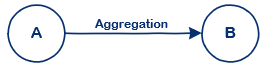
\includegraphics[width=0.45\textwidth]{figs/fig-aggregation.png}
}

\item{
	\lr{Composition}:
	بین کلاس A و کلاس B رابطه ترکیب وجود دارد. یک یا چند شیء از کلاس B در کلاس A تعریف شده است و نمونه‌های B به نمونه‌های A وابسته‌اند.
	
	
\includegraphics[width=0.45\textwidth]{figs/fig-composition.png}
}
\end{enumerate}

ابزارهای متعددی برای مصورسازی کد و استخراج نمودار ارتباطی کلاس‌ها از کد منبع برنامه آنها وجود دارد 
\cite{EA2020,VP2020,Understand2020}.
این ابزارها زبان‌های برنامه نویسی متداول را پشتیبانی می‌کنند. اما نمودار کلاس UML بایستی مورد پیش‌پردازش قرار گرفته و گراف ارتباطی کلاس‌ها از آن استخراج شود؛ زیرا، در نمودار کلاس اطلاعات بیش‌تری مانند نوع و نام فیلد‌ها وجود دارد که در اینجا به آنها نیاز نداریم. 
استفاده از هر ابزاری برای تولید گراف در این قسمت مجاز است.
برای نمونه ابزار 
\lr{Enterprise Architect} \cite{EA2020}
به آسانی نمودار کلاس را از کد منبع یک برنامه تولید کرده و آن را در قالب \lr{XMI}
که خود نوعی فایل \lr{XML} است، به‌عنوان خروجی می‌دهد. با خواندن و پردازش این فایل، گراف ارتباطی برنامه قابل ایجاد است. یک نمونه برنامه تجزیه‌گر برای فایل‌های \lr{XMI} در 
\cite{XMI2020}
 آمده است که عملیات استخراج اطلاعات از این فایل را با فراهم آوردن \lr{API} مناسب تسهیل می‌کند. 


\subsection{تولید گراف ‌الگوهای طراحی}
نمایش گرافی ارتباط کلاس‌ها این ویژگی‌ را دارد که مستقل از زبان برنامه‌نویسی است. الگوهای طراحی نیز ذاتاً مستقل از برنامه هستند و گراف آنها را می‌توان از پیاده‌سازی آنها استخراج کرد. پیاده‌سازی جامعی از الگوهای طراحی مهم با زبان \lr{C++} در 
\cite{RefactoringGuru2020}
آمده است. همچنین در همین منبع شرح کامل هر الگوی طراحی، آورده شده است. پیاده‌سازی دیگری نیز در آمده است
\cite{Wikibooks2020}. 
برای هر الگوی طراحی گراف نظیر آن، مشابه بخش \ref{sec:code2graph}، قابل تولید است.


\subsection{یافتن الگوهای طراحی در نرم‌افزار}
هر نرم‌افزار شی‌گرا ممکن است از یک یا تعدادی از الگو‌های طراحی استفاده کرده باشد. این الگوهای طراحی استفاده شده به‌صورت زیرگرافی\LTRfootnote{sub-graph} در گراف اصلی برنامه، وجود خواهند داشت.
 در این صورت با جست‌وجوی گراف مربوط به هر الگوی طراحی در گراف اصلی و تطبیق یک زیرگراف یافت شده با آن الگوی طراحی، استفاده یا عدم استفاده از این الگو در گراف مشخص می‌شود. تشخیص الگوها صرفاً با استفاده از یک‌ریختی گراف\LTRfootnote{Graph isomorphism}، دقیق نبوده و همان‌طور که گفتیم قابل بهبود است. با این حال در این مرحله هدف استفاده تطبیق گراف الگوهای طراحی با زیرگراف‌هایی از گراف اصلی برنامه و تعیین الگوها است.
 
 
 \subsection{پروژه - فاز اول}
مراحل زیر را انجام داده، ابزارها و گزارش‌های خود را در ارتباط با هر گام تحویل دهید:

\begin{enumerate}
	\item{
	گراف ارتباطی کلاس‌ها را برای پیمانه‌های
	 \lr{control}\footnote{\href{https://github.com/ApolloAuto/apollo/tree/master/modules/control}{https://github.com/ApolloAuto/apollo/tree/master/modules/control}}
 و 
 \lr{planning}\footnote{\href{https://github.com/ApolloAuto/apollo/tree/master/modules/planning}{https://github.com/ApolloAuto/apollo/tree/master/modules/planning}}
 سیستم اتومیبل خودران 
 \lr{Apollo} \cite{Apollo2020}،
 استخراج نمایید.
	}

\item{
ویژگی‌های اولیه گراف، مانند توزیع درجه و گره‌های مرکزی را برای گراف هر کدام از پیمانه‌ها مشخص نمایید. با تحلیل نتایج مهمترین کلاس‌های هر کدام از پیمانه‌ها را تعیین کنید.

}

\item{
	گراف ارتباطی کلاس‌ها را برای الگوهای طراحی در \cite{RefactoringGuru2020}، به‌دست آورید.
	
}

\item{
	الگوهای طراحی استفاده شده در هر کدام از پیمانه‌های 
	\lr{control}
	و 
	\lr{planning}
	را مشخص و گزارش نمایید.
}

\item{
	با تعیین نسبت تعداد کلاس‌هایی که عضوی از یک الگوی طراحی بوده‌اند به تعداد کل کلاس‌های برنامه (پیمانه)، کیفیت آن پیمانه را محاسبه کنید.
}

\item{
	نقاط ضعف و قوت روش خود در هر گام را توضیح دهید.
}
 
 
\end{enumerate}


\section{استخراج معماری}\label{sec:extract-architecture}
مهندسی معکوس کد و استخراج معماری از کد منبع برنامه (به بیان دقیق تر استخراج مدل ارتباطی کلاس ها و تعیین طرح معماری نرم افزار) عمدتاً با سه رویکرد صورت می پذیرد. نخست، تولید مستندات از متن برنامه موجود و از پیش نوشته شده، به منظور نگهداشت و توسعه آن. دوم، کشف ساختار کدهای حجیم به منظور درک عملکرد آن ها و تأثیرشان بر روی سیستم های کامپیوتری و سوم سنجش کیفیت نرم‌افزار. یک روش دیگر برای سنجش کیفیت معماری نرم‌افزار، اندازه‌گیری پیمانگی
\LTRfootnote{\lr{modularity}}
 است. چسبندگی 
\LTRfootnote{\lr{cohesion}}
 و اتصال 
\LTRfootnote{\lr{coupling}}
 دو اصل حاکم بر پیمانه‌ها در نرم‌افزار هستند. در یک پیمانه‌بندی خوب شاهد پایین بودن اتصال و بالا بودن چسبندگی هستیم. این مفاهیم دقیقاً همان مفاهیم مطرح در تشخیص جوامع در شبکه‌های پیچیده هستند. اصول یادشده بر این نکته تأکید دارند که ارتباط بین گره‌ها داخل یک جامعه زیاد و ارتباط بین گره‌ها بین دو جامعه متمایز کم است. بنابراین هدف بسته‌بندی کلاس‌ها داخل پیمانه‌های مختلف است به نحوی که اختلاف چسبندگی و اتصال بیشینه شود.
 

\subsection{تعیین پیمانه‌ها}
با استخراج گراف ارتباطی کلاس، امکان استخراج پیمانه‌ها از طریق روش‌های خوشه‌بندی گراف و تشخیص جامعه میسر می‌شود. برای این منظور می‌توان از گراف به‌دست آمده در بخش  \ref{sec:design-pattern-extraction}، استفاده کرده و عملیات خوشه‌بندی را بر روی‌ آن انجام داد. الگوریتم‌های مختلفی برای تشخیص جامعه، در حوزه شبکه‌های پیچیده ارائه شده است. می‌توان تعدادی از این الگوریتم ها را استفاده و نتایج را با یکدیگر مقایسه کرد. یک روش و ابزار برای این منظور در 
\cite{Mancoridis2006, Mancoridis1999}
معرفی شده است.



\subsection{پروژه - فاز دوم}
مراحل زیر را انجام داده و ابزارها و گزارش‌های خود را تحویل دهید:

\begin{enumerate}
	\item{
		با استفاده از خوشه‌بندی گراف ارتباطی استخراج شده در فاز اول پروژه برای پیمانه‌های   \lr{control} و \lr{planning}، معماری هرکدام را در سطح نمودار مؤلفه پیدا کرده و میزان پیمانگی را مشخص نمایید.
	}

\item{
	میزان پیمانگی را برای معماری فعلی هرکدام از پیمانه‌های  \lr{control} و \lr{planning}، محاسبه کنید. میزان بهبود پیمانگی با روش پیمانه‌بندی خودکار چه‌قدر است؟ 
}

\item{
	گراف ارتباطی را بدون جهت در نظر بگیرد و گام‌های (1) و (2) را انجام دهید. نتایج را با گام (1) مقایسه کنید.
}

\item{
	\textbf{(اختیاری) }
	گراف ارتباطی را به‌صورت جهت‌دار و وزن‌دار در نظر گرفته و مراحل را تکرار کنید. وزن هر یال در این حالت برابر با تعداد ارتباطاتی است که از کلاس اول (فراخواننده) به کلاس دوم (فراخوانده شده) وجود دارد. یک نمونه از این کار در 
		\cite{Mancoridis2006}
	انجام شده است. نتایج این گام را گام‌های قبلی مقایسه کنید. 
}


\item{
	\textbf{(اختیاری) }
	برنامه‌ای بنویسید که گراف مؤلفه‌های استخراج شده و کلاس‌های داخل هر یک را به یک فایل \lr{XMI} تبدیل کند به نحوی که توسط نرم‌افزار  
	\lr{Enterprise Architect} \cite{EA2020}
	باز شود. با این کار، مرحله طراحی در فرایند مهندسی نرم‌افزار را به‌طور کامل خودکار نموده‌ و یکی از مراحل این فرایند را حذف کرده‌اید.
}

\item{
	نقاط ضعف و قوت روش خود در هر گام را توضیح دهید.
}

\end{enumerate}


\section*{تحویل پروژه}
\label{sec:deliver-project}
\addcontentsline{toc}{section}{\nameref{sec:deliver-project}}
یک قالب گزارش \lr{LaTex} از طریق لینک زیر
در اختیار شما قرار داده می‌شود که برای هریک از گام‌های موجود در پروژه یک فضا در نظر گرفته است. شما بایستی آن را تکمیل نموده و تحویل دهید.
موعد تحویل پروژه نیز اطلاع رسانی خواهد شد. در صورتی که مشکلی در نگارش این سند وجود داشت و یا مطلبی برای شما مبهم بود می توانید از طریق نشانی ایمیل 
\lr{\href{mailto:m-zakeri@live.com}{m-zakeri@live.com}}
درخواست و یا پرسش خود را ارسال فرمایید.

\noindent$\lhd$
دریافت قالب گزارش:

{\centerline{
\lr{\href{https://www.dropbox.com/s/bwb9yuq4rapv9mx/report_template_project1.zip?dl=0}{https://www.dropbox.com/s/bwb9yuq4rapv9mx/report\_template\_project1.zip?dl=0}}
}}



\clearpage
\thispagestyle{plain}
\fancyhead[LO,RE]{\slshape }
\onehalfspacing
\bibliographystyle{ieeetr-fa}%{acm-fa}%{chicago-fa}%{plainnat-fa}%
\bibliography{bibitems/references-all.bib}

\end{document}